\section{Production Simulation}
\label{sec:productionSim}
 \begin{quotation}
"Production is a process of combining various material inputs and immaterial inputs (plans, know-how) in order to make an output for consumption. It is the act of creating an output, a good or service which has value and contributes to the utility of individuals."\cite{noauthor_production_2019}
 \end{quotation}
The definition above provides us with the basis of the production process. In it we can already start to differentiate separate sectors, such as the Procurement Department for getting the material inputs and the HR department for providing the know-how, the human factor in production. \\
In this simulation we are going to focus on three very important indicators, namely product quality, product cost, production performance. In order to derive these indicators we will need to analyze the factors that influence them and give them proper values. 

Firstly, product quality is considered a very important element in the production simulation, nevertheless it is a very volatile concept and thus challenging to define and implement in this simulation. Often defined as conformance to requirements \cite{crosby_quality_1979}, quality is an elusive factor of production, which we have tried to frame in order to serve the scope of this project.

 Several factors that affect product quality in our CapitalismX simulation are listed below:
\begin{itemize}
\item Production Technology (PT)
\item Production Employee Skills (PES)
\item Procurement Quality (ProcQ)
\item Logistic Quality (LQ)
\item R\&D
\end{itemize}
Product quality is influenced by many elements, that in principle belong to the extend of other departments in the company. To illustrate, employee skills are included in the HR simulation, the supplier index is included in the procurement simulation, logistics and warehousing in their respective simulations, etc. \\
These elements all correlate in order to give an estimation of product quality.
All the elements have a $5$ point Likert-Scale, except from the supplier indexes.
These indexes, namely Eco-Index of the supplier $(EI_{s})$ and the Base Quality of the supplier $(BQ_{s})$ have a scale of measurement of $3$ points. They vary from good, medium to bad. In order to handle this divergence in scale, we have adjusted the supplier indexes by multiplying their sum with $\frac{5}{6}$. These indexes will be attributed to the total Procurement Quality.
\begin{equation}
ProcQ=(EIs + BQs)\times \frac{5}{6}
\end{equation}

In order to converge all the above mentioned elements and to measure Product Quality, we have compiled the following equation.
\begin{equation}
ProductQuality = (PES+PT+R\&D+LQ +ProcQ) \times 0.04_{N\footnotemark}
\label{eq:PQ}
\end{equation}
\footnotetext{N: index is normalized in the range of $[0-1]$}
 
After giving you an understanding of our concept of product quality, in the following sections we will explain the elements that  are included in this formula, and also further concepts that apply to the production process.

\subsection{Production Technology Level}
We will focus on Production Technology in this chapter, as you will encounter all the other elements in the following simulations. \\
Table \ref{table:my-label}, explains the $5$ points Likert-Scale for measuring Production Technology. This scale has a range of $[1-5]$, where $1$ is the lowest value and $5$ the highest.

\begin{table}[ht]
\centering
\begin{tabular}{|c|l|}
\hline
 Range & Production Technology\\
\hline
 1 & Depreciated  \\
 2 & Old \\
 3 & Good conditions \\
 4 & Purchased more than 5 years ago  \\
 5 & Brand New\\
\hline
\end{tabular}
\caption{Production Technology}
\label{table:my-label}
\end{table}

The technology of the machinery used in production starts at level $5$, when all machinery is new. This level can change during the game, by either increasing or decreasing. The Production Technology level can decrease one level$(-1)$ over a $5$ years time-span, due to the effects of machine depreciation. This index can decrease two levels$(-2)$, if a natural disaster such as a fire, flood or a hurricane occurs.\\
There are also possibilities to improve the production technology level after a certain period of time has passed. These actions are created to  positively influence the technology level of machinery.
\begin{itemize}
    \item Purchasing new machinery (level $5$) \\
		Purchasing new machinery immediately sets the machine's technology level to $5$, the maximum level, because the machinery is new and it complies with the measures of eco-laws and safety regulations.
\item Maintaining \& repairing $(+1)$ \\
Maintaining a machine is a regular process in all production companies. In CapitalismX, maintenance is optional for each machine, and the player can select which machine to maintain for a certain price. The price for maintenance is fixed for every machine and it improves the Production Technlolgy scale by one level. 
Repairs are also very frequent processes in production companies. Machines do not always function properly, and after using them at full capacity for a period of time they need intervening actions in order to restore them into their optimal state. In this simulation, repairs also increase the production technology scale by one level, as repairing is necessary, but it does not offer additional features to the machine.
\item Upgrading ($+2$) \\
Upgrading a machine is a process that implements new, better features into the current machine. Alongside with increasing the production technology scale by two levels, upgrading also allows increasing the individual machine production capacity by $20\%$.
\end{itemize}
When buying a new machine the prices will be set by the game mechanics. This price calculation will be decided on the capacity of each machine, since they will all have a production technology level equal to $5$. The supplementary $20\%$ of the price is added to the amount, as an additional payment for the retailer.
\begin{equation}
buyMachinePrice=(1000cc+MC)\times 120\%
\label{eq:buyMachine}
\end{equation}
In this simulation it is also possible to sell your current machines. A player should choose this option if he is low on CapCoins, or has purchased too many machines and they are deteriorating. The selling price will be set by the game mechanics, accordingly with equation \ref{eq:sellMachine}.
\begin{equation}
sellMachinePrice=(PT \times 200cc)+MC
\label{eq:sellMachine}
\end{equation}
\begin{center}
	where\\
	PT = Production Technology level \\
	MC = Machine Capacity
\end{center}
In this formula, the selling price is calculated by multiplying the current production technology with a bench-marked value of $200cc$ and adding the capacity value. It is formulated as such because when the player purchases a machine its cost varies in terms of capacity. Whilst, when selling a machine not only the capacity changes between machines but also the production technology level.

\subsection{Production Investments}
The player can decide how to improve Production Performance based on several investment options. These investments are correlated with the measurements of several performance indicators, in the production simulation. The player has to use his instinct and business intuition in order to understand which metric do these investments influence and how. It is the player's decision to insert the amount of Cap-Coins(cc), that he wants to invest. \\
The available investment possibilities are:
\begin{itemize}
\item Research and Development (R\&D)
\item System Security
\item Process Automation (PA)
\end{itemize}
These investments options are also measured in our standard $5$ points Likert-Scale. The difference in these options lies in the fact that they start at level $1$, considering that in the beginnings the company has no investments operating. The increase or decrease of these indexes is dependent on the amount of CapCoins that is invested in them.

\begin{table}[ht]
\centering
\begin{tabular}{c|c|c}
\hline
 Level & Description & CapCoins$_{(cc)}$\\
\hline \hline
 1 & No Investment & $100cc$ \\
 2 & Bad & $ 500cc$\\
 3 & Normal & $1000cc$ \\
 4 & Good & $1500cc$ \\
 5 & Very good & $2000cc$\\
\hline
\end{tabular}
\caption{Levels of Production Investments}
\label{table:prod-investments}
\end{table}
As illustrated in Table \ref{table:prod-investments}, all three of these indexes will be able to change their current level by investing the corresponding amount of money.\\
Despite these investments being made once, there will come to a point in time, when they will begin loosing their added value to the production process. This loss is represented by Figure \ref{fig:InvestmentGraph}, and its corresponding function is $f(x)=5\times\exp^{-x}$. We take in consideration the $x$ range from $0$ to $10$. This graph encompasses the phenomena of "loss of added value" that we wanted to convey.

\begin{figure}[ht]
\centering
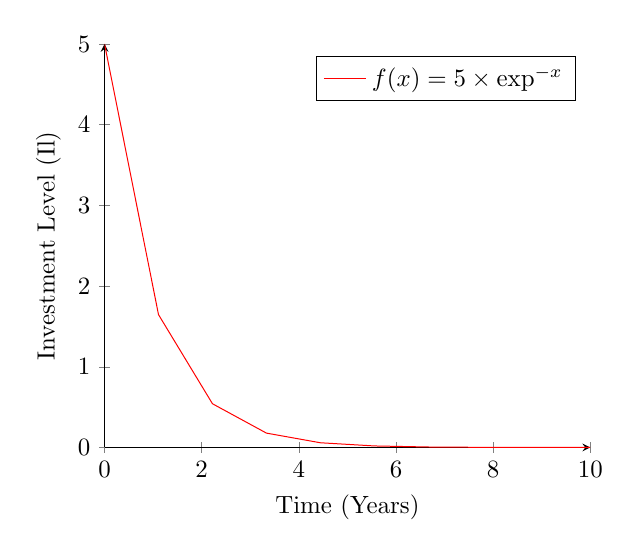
\begin{tikzpicture}[scale=0.9]
\begin{axis}[
    axis lines = left,
    xlabel = Time (Years),
    ylabel = Investment Level (Il),
    grid style = dashed,
    legend pos=north east
]

\addplot [
    domain=0:10, 
    samples=10, 
    color=red,
]
{5*e^(-x)};
\addlegendentry{$f(x)=5 \times \exp^{-x} $}
\end{axis}
\end{tikzpicture}
\captionof{figure}{\textbf{Production Investment Graph}}	\label{fig:InvestmentGraph}
\end{figure}


In order to avoid the investments to significantly lower product quality, the player must keep in mind to invest in these elements constantly over the duration of the game. Preferably, the investments should be less than $5$ years apart, since the effect of the investment reaches $0$ after this time-span.\\
There is a special event, we have implemented regarding System Security.
If the system security indicator falls below the $3^{rd}$ level threshold, incidents in the workplace and stealing inside the company will start to occur and they will negatively influence Company Image. \\
Process Automation is another investment option and it represents the company's investments towards more automated, futuristic processes. Its range is the same as the other investments and is set by the amount of money invested. We will expand this concept in section \ref{sub:PM}.
All the simulation explained in this section will not be visible to the player, in order to increase the level of difficulty of the game and make the player more perceptive to the effect of these elements. 


\subsection{Production Costs}
\label{prodCosts_simulation}

To determine the total product cost, several components have to be taken into account, as demonstrated in Figure \ref{fig:productionCosts}. The first is CP which is the sum of all component costs, since we need several components in order to have one end product. The overall employee salary would be included in the equation since all employees no matter in which department they work in, give an input and add value to the product. But we have decided to separate costs according to departments, that is why employee salary will be included in the HR costs. Another cost that we have included in our simulation is the eco-cost. You can find the details regarding eco-cost calculation in section \ref{sec:compEco-idex}. Furthermore we have incorporated machinery costs, since machinery is purchased, maintained and upgraded, we have to account these expenses to machinery costs, which are part of fixed costs. Fixed costs (FC) like electricity, depreciation costs or rent are also included because they are inevitable expenses that are present in every production company. 

\begin{figure}[ht]
	\centering
		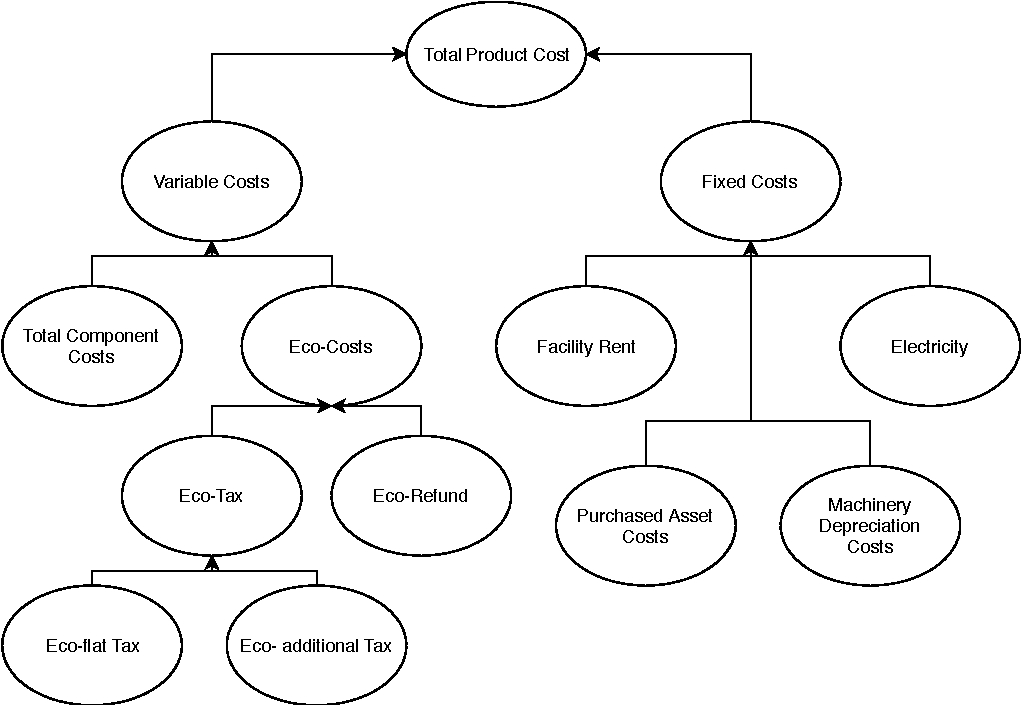
\includegraphics[scale=0.55]{images/ProductCost.pdf}
	\caption{Production Costs}
	\label{fig:productionCosts}
\end{figure}
All the above mentioned costs, add up to two major categories, variable costs and fixed costs. Together they compose the total product cost.\\
 In function \ref{eq: PC/u}, we sum up $5$ component prices, as each product can only have $5$ components per unit. In order to complete the product cost, the eco-cost and fixed costs were added and divided by the number of units in order to get a standardized dependent variable.
\begin{equation}
	Product Cost_{per Unit}= \sum_{n=1}^{n=5}CP + (\frac{Eco–Cost}{nr. Units}) + (\frac{FC}{nr. units}) 
	\label{eq: PC/u}
\end{equation}
By observing the above equation, we have described how the costs are simulated in the production process. 

\subsection{Performance metrics}
\label{sub:PM}
In this section we are going to present some important metrics that help us understand how, not only quality but also production performance is measured in our game. In order to measure production performance there are several other metrics that need to be defined. \\
Equation \ref{eq: PES} shows the calculation of production employee skills. This calculation is a weighted average of the level of Process Automation and Employee Skills, which are defined in chapter \ref{sec:HRsim}. As you can notice more weight has been given to Employee Skills as it is a more relevant factor in determining our dependent variable. Process Automation on the other hand is a bit more complex as it needs to have some prerequisites fulfilled regarding employee skills. In order to increase PA according to the money invested, the player must have trained the employees in the production area, which means that the new technologies that will be implemented in production, will meet with employees that are trained to handle them. The possible trainings can be seen in section \ref{sub:KPI}. It is required to have at least $1$ production engineer trained, for each level of PA. For instance, in order to invest and have PA set in level $4$, at least $4$ production employees need to be trained in the production area.
\begin{equation}
Production Employee Skills= 0.4\times PA + 0.6\times ES
\label{eq: PES}
\end{equation}

Manufacture efficiency is measured by dividing the number of goods produced, on a daily basis, by the current number of machines times their average capacity to produce. This measure is important as it shows the player the rate in which the machinery is being utilized. This index has a range of $[0-1]$,which means if ME is close to $1$ the usage of the machinery is optimal, but if this index is low, the player should realize he should either produce more or sell some of the machinery in order to keep efficiency high and not waste resources.
\begin{equation}
ME= \frac{nr. units Produced(daily)}{nr. Machines\times avg. Capacity}  
\label{eq: ME}
\end{equation}

Production Process Productivity (PPP) is an indicator of the efficiency of our production  process. It is based on Production Technology and Production Employee Skills as indicators of the quality of the process and Manufacture Efficiency as an indicator of the efficiency of the manufacturing process.
\begin{equation}
PPP= [(PT + PES) \times ME]/10_{N\footnotemark}
\label{eq:PPP}
\end{equation}
\footnotetext{N: index is normalized in the range of $[0-1]$}
 
To conclude, in our production simulation we explained several elements that influence the production process. These elements include machinery, possible investments and performance metrics. All of these elements derive to the two most important indicators, which are product quality and production process productivity. By creating these indicators we have scratched the surface of manufacturing as a process, but they provide a strong basis in order to provide a successful Production Simulation. 